%%%%
\section{África}

Os maiores níveis de poluição de ar no mundo ocorre
em cidades da Ásia, África e Oriente Médio \citep{brauer2012}.   

A poluição do ar ambiental nas cidades dos países em desenvolvimento 
guarda algumas similaridades com as dos países desenvolvidos, já que 
possuem algumas fontes poluídoras características de meios urbanos, 
tais como, tráfego de veículos automotivos, industrias, geração de 
eletrecidade por usina hidrelétrica ou termelétrica, entre outras. 

Entretanto, nas cidades dos países em desenvolvimento, é comum 
a população encontrar outros meios para geração de energia quando 
o Estado não atende as demandas urbanas de infraestrutura, assim o 
uso queima da biomassa para cozimento de alimentos em residências 
e comércio, uso de querosene para iluminação noturna, frota veicular
com tecnologias ultrapassadas, entre outras, fazem com que o perfil 
de fontes poluídoras dessas cidades sejam significativamente 
diferentes das cidades dos países desenvolvidos \citep{brauer2012}.

Em 2015, a África contava com $1.186,178$ habitantes, ficando atrás 
apenas da Ásia, que possuia $4.393,296$ habitantes no mesmo período. 
Possui área territorial de 30 milhões de quilômetros quadrados, sendo
o terceiro maior continente em extensão, contando com 54 países 
independentes \citep{UN}.

Devido seu tamanho e extensão, possui grande diversidade social, 
econômica, climática, geográfica e política. 
Há entretanto, uma barreira natural formada pelo \textbf{Deserto do Saara}
separando norte e sul da África. Separação não só geográfica, como
social, étnica, econômica etc. 
A África Subsariana \textbf{(SSA)}, localizada ao sul do \textbf{Deserto do Saara}, 
conta com os países maios pobres do mundo, mas que ao mesmo tempo estão
passando por um processo intenso de urbanização \citep{UN}. 
   	
%%%%
\subsection{África Subsariana \textbf{(SSA)}}

A África Subsariana \textbf{(SSA)}, localizada ao sul do 
\textbf{Deserto do Saara}, é atualmente a região no mundo que tem a maior 
taxa de transição da população rural - ainda predominante - para cidade. 
As regiões rurais não são atendidas por eletrecidade \citep{MONTGOMERY2008}.

Até 2003, nenhuma cidade da \textbf{SSA} possuia sistemas de monitoramento 
sistemático de poluição do ar e medidas esporádicas foram até então realizadas
de cunho acadêmico e não governamental, mas que tem relevado, concentrações
de poluentes acimas dos recomendados pela Organização Mundial de Saúde \textbf{OMS} 
\citep{EZZATI2004}. 

Diferente dos países industrializado, onde as principais fontes de poluição 
são os setores da industria e do transporte, nos países da \textbf{SSA} a 
queima de biomassa assume a primazia, sendo comum o seu uso no cozimento 
de alimentos, tanto em regiões urbanas quanto rurais \citep{SMITH2004}. 

Destaca-se características regionais da \textbf{SSA} que ampliam as diferenças 
na do perfil de fontes poluídoras do ar comparada com cidades de países desenvolvidos: 

\begin{itemize}
  \item População predominantemente rural;
  \item Muitas vias não pavimentadas;
  \item Maior taxa de crescimento populacional urbano do mundo;
  \item População jovem;
  \item Não possuem sistemas de monitoramento sistemático de Poluição do Ar em larga escala;
  \item Uso da queima de biomassa nas residências e comércio para o cozimento de alimentos,
        tanto em regiões urbanas quanto rurais.
\end{itemize}

%%%%
\subsection{Gana}

O Gana situa-se na África, 5 graus a norte do Equador, portanto possui clima
equatorial. Faz fronteira a oeste com a Costa do Marfim, ao norte com Burkina 
Faso e ao leste pelo Togo. 

As chuvas ocorrem em dois períodos, entre Maio e Junho e entre Agosto e Setembro.
Um vento quente e seco provindo de nordeste sopra entre final de Dezembro
e início de Fevereiro e é chamado de Harmatão. O Harmatão vem carregado de 
poeira do \textbf{Deserto do Saara} \citep{breuning2005}.

O \textbf{United States Department of Commerce National Oceanic 
and Atmospheric (NOAA)} mantém um banco de dados com parâmetros 
meteorológicos do mundo inteiro enviado por estações meteorológicas 
cadastradas \citep{noaa}. 

Utilizando-se os dados horários de Setembro de 2006 à Junho de 2008 
coletados na estação meteorológica do aeroporto de Acra 
(\textbf{Kotoka International Airport}) cadastrado na \textbf{NOAA},
pode-se verificar através do gráfico de distribuição de frequência de
direção dos ventos (\ref{fg:windFrequencyCompleto}) que a direção 
predominante de origem dos ventos é sudoeste.
 
\begin{figure}[H]
  \centering
  \includegraphics[width=0.5\textwidth]{../outputs/completo2006_2008.pdf}
  \caption{Distribuição da frequência do vento em (\%) entre
           Setembro de 2006 e Junho de 2008. Utilisou-se dados 
           do \textbf{Kotoka International Airport} de Acra \label{fg:windFrequencyCompleto}}
\end{figure}

Pode-se incluir a intensidade do vento nessa análise e plotar a
clássica rosa dos ventos (\ref{fg:rosaCompleta}). Nota-se que os ventos
mais intensos (com mais de 10 m/s) são também de sudoeste. 

\begin{figure}[H]
  \centering
  \includegraphics[width=0.5\textwidth]{../outputs/windRoseNoaaHarvard.pdf}
  \caption{Rosa do ventos entre
           Setembro de 2006 e Junho de 2008. Utilisou-se dados 
           do \textbf{Kotoka International Airport} de Acra \label{fg:rosaCompleta}}
\end{figure}

A distribuição de frequência por estação do ano pode ser vista em 
\ref{fg:windFrequencyStation}. 
No inverno, quando há ocorrência do Harmatão, esperaria-se maior
frequência de ventos de nordeste, mas no gráfico do inverno é quase 
impercepitível esse aumento. \citep{breuning2005} mostra que na 
verdade o vento do Harmatão passa por Gana em altas altitudes, por isso
não influência os ventos locais. 

\begin{figure}[H]
  \centering
  \includegraphics[width=0.4\textwidth]{../outputs/windFrequencySpring.pdf}
  \includegraphics[width=0.4\textwidth]{../outputs/windFrequencySummer.pdf}
  \includegraphics[width=0.4\textwidth]{../outputs/windFrequencyFall.pdf}
  \includegraphics[width=0.4\textwidth]{../outputs/windFrequencyWinter.pdf}
  \caption{Distribuição da frequência do vento em (\%) entre
           Setembro de 2006 e Junho de 2008 por estação do ano. Utilisou-se dados 
           do \textbf{Kotoka International Airport} de Acra \label{fg:windFrequencyStation}}
\end{figure}

Os últimos dois censos demográficos realizados em Gana datam
de 2000 \citep{ghanacensus2003} e 2010 \citep{ghanacensus2013}. Os
dados resultantes podem ser encontrados no portal de dados abertos
do Governo Federal de Gana \citep{opendataghana}.

A população de Gana em 2000 correspondia a $18,9$ milhões 
de habitantes e em 2010 subiu para $24,7$ milhões, tendo assim
um aumento de $30\%$ no intervalo dos dois censos demográficos.

No censo demográfico de 2010, indica que $49\%$ da população está 
no meio rural e $61\%$ no meio urbano. As mulheres representam 
$51,2\%$ da polulação.

A pirâmede etâria de Gana \ref{fig:piramedegana} indica população jovem, 
e que a expectativa média de vida está não é muito maior que 50 anos. 

\begin{figure}[H]
\begin{center}
  \includegraphics[width=0.5\textwidth]{../outputs/piramide_etaria.pdf}
  \caption{Pirâmide etária Gana plotada com dados do censo 
           demográfico de 2010 \citep{ghanacensus2013} \label{fig:piramedegana}}
\end{center}
\end{figure}

A economia de Gana, antes essencialmente dominada pela agricultura, 
agora está distribuída entre: industria $19\%$, agricultura $30\%$ 
e serviços $51\%$ \citep{ghanacensus2013}.
Na industria, recebe destaque fabricação e exportação de aparelhos digitais, 
automóveis e navios. Em termos de matéria primária, há grande exportação de 
hidrocarbonetos e minerais \citep{ghanacensus2013}.

O produto interno bruto (PIB) per capita anual de Gana em 2010 foi
de \$ 1.323,09 USD e no Brasil no mesmo ano \$ 11.124,09 USD.
O gráfico da figura \ref{fib:pib} apresenta o \textbf{PIB} de Gana e do Brasil 
calculado pelo Banco Mundial \citep{bancomundial}.

\begin{figure}[H]
\begin{center}
  \includegraphics[width=0.5\textwidth]{../outputs/PIBGhanaBrazil.pdf}
  \caption{\textbf{PIB} do Brasil e de Gana. Plotado com dados do 
           Banco Mundial \citep{bancomundial} \label{fig:pib}}
\end{center}
\end{figure}

A responsabilidade do controle, fiscalização e monitoramento das 
atividades poluídoras em Gana é realizado pela 
\textbf{Ghana Environmental Protection Agency (EPA Ghana)}, que é 
hierarquicamente subordinada ao 
\textbf{Ministério de Meio Ambiente, Ciência, Tecnologia e Inovação} do 
Governo Federal de Gana.

%%%%
\subsection{Região Metropolitana de Acra \textbf{(RMA)}}

Acra é uma cidade litorânea e é a capital de Gana. Está localizada 
no Golfo Guiné tendo área total de mais de 2500 $km^2$, com elevações que 
variam de 0 até 60 metros do nível do mar \citep{ARKU2008}.

A Região Metropolitana de Acra \textbf{(RMA)} agrega outras 9 cidades
além de Acra e conta com uma população total de 4 milhões de habitantes. 
Se caracteriza por ter sua economia baseada exclusivamente na industria 
e em serviços, $90,5\%$ da polulação ocupando o meio urbano \citep{ghanacensus2013}.

Em 2010, havia aproximadamente 1000 fazendas urbanas com produção de vegetais 
para consumo local em Acra, onde as irrigações são feitas por água não tratada, 
provinda de córregos locais. Altos indíces de metais pesados 
(Fe, Mn, Cu, Zn, Pb, Ni, Cr, Cd, Co) foram encontrados nas plantações 
dessas fazendas \citep{lente2014}, pois os resíduos das residências são despejados 
diretamanente nos córregos.

A densidade populacional em \textbf{(RMA)} é de 1205 $habitantes/km^2$, 
enquanto que na Região Metropolitana de São Paulo \textbf{(RMSP)} é de 
2476 $habitantes/km^2$ \citep{ibge2011}. 

\textbf{Driver and Vehicle Licensing Authority (DVLA)} é o
departamento do governo de Gana que cuida dos registros de automóveis, 
mas há muitos automóveis circulando que não são registrados. 
Em contava em 2009, Gana contava com 1,12 milhões de veículos legais. 
Na tabela \ref{table:dvla} percebe-se que a frota dobrou em um década.

\begin{table}[H]
 \centering
  \input{../outputs/frota_ghana.tex}
  \caption{Frota veícular de Gana \citep{dvla} \label{table:dvla}}
\end{table}

Segundo a EPA de Gana \citep{epagh} as fontes de poluição do ar ambiental 
majoritárias em Acra, são:

\begin{itemize}
  \item Emissões veiculares, principalmente emissões de veículos antigos sem manutenção;
  \item Emissões industriais;
  \item Queima de lixo e outros materiais a céu aberto;
  \item Poeira de ressupensão de solo, pois há muitas vias ainda não pavimentadas;
  \item Vento seco do \textbf{Deserto do Saara}, o harmatão.
\end{itemize}

%%%%
\subsection{Nima}

O bairro análisado foi \textbf{Nima}, que tem por características
ser um bairro dormitório de Acra. O principal meio de transporte
dos trabalhadores de Nima para a zona industrial e de serviços de Acra é 
feito por vans. Muitas vias não são pavimentadas e a intensa movimentação
de veículos causa ressuspensão de poeira do solo, já que há vias não
pavimentadas.

O carvão e a lenha são as principais fontes de energia para cozimento 
em Nima. Na figura \ref{fig:nima} há imagens mostrando como as cozinhas
são equipadas. 

\begin{figure}[H]
  \centering
    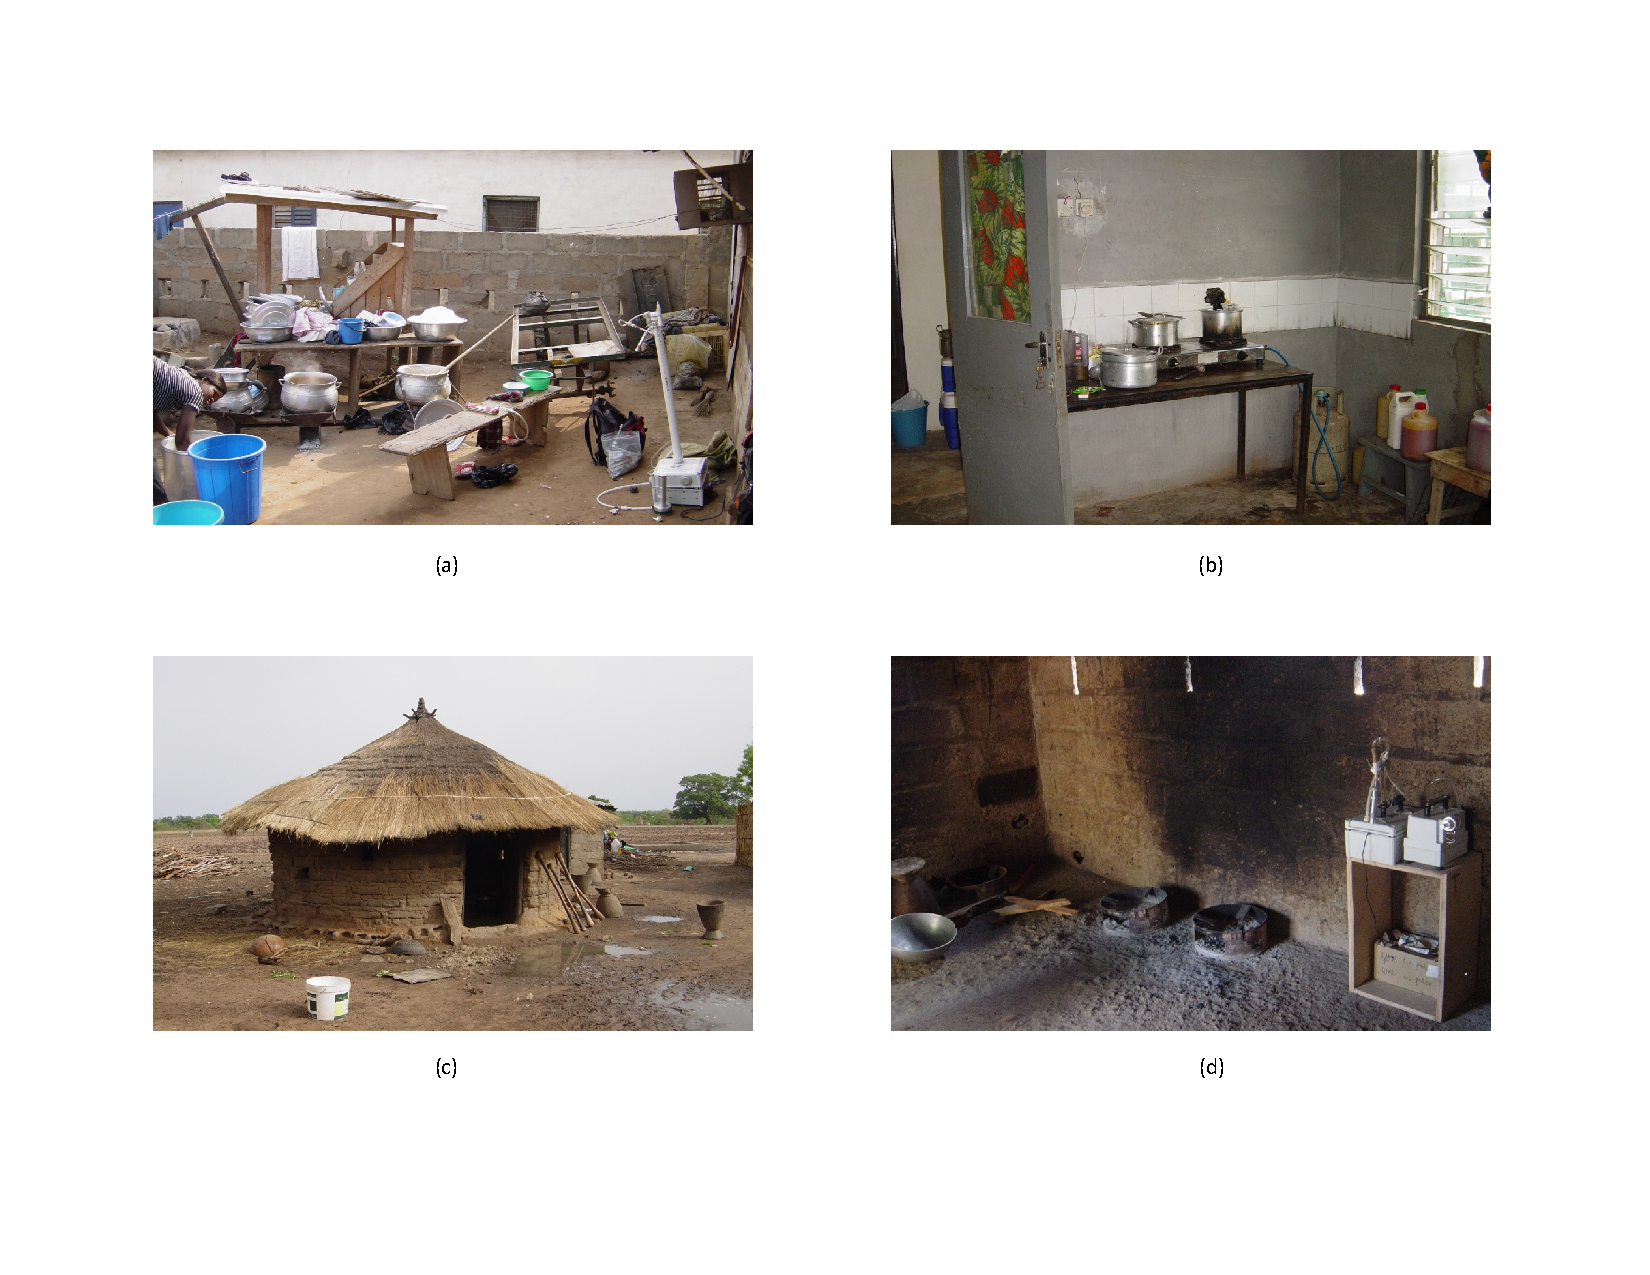
\includegraphics[width=0.7\textwidth]{../inputs/images/zheng/nima.pdf}
    \caption{Fotos de residências de Nima, por Raphael Arku \label{fig:nima}}
\end{figure}

Foi feito um levantamento das principais fontes poluídora de Acra.
Na figura \ref{fg:acrasources} estão assinalados os dois pontos de 
amostragem em Nima, fontes poluídoras levantadas, bem como a aeroporto
(onde foram coletados os dados meteorológicos).

\begin{figure}[H]
  \centering
  \includegraphics[width=0.9\textwidth]{../outputs/accra_sources.pdf}
  \caption{Levantamento de algumas fontes poluídora de Accra \label{fg:acrasources}}
\end{figure}

Acra é mundialmente conhecida por receber ilegalmente lixo 
eletrônico dos países desenvolvidos, que são então derretidos, de forma
imprópria, para obtenção de cobre pela população local. 
O depósito de lixo eletrônico, conhecido como \textbf{e-waste}, 
fica no bairro \textbf{Agbogbloshie}, $4 km$ a sudoeste de \textbf{Nima}
\citep{asampong2015}.

\begin{figure}[H]
  \centering
  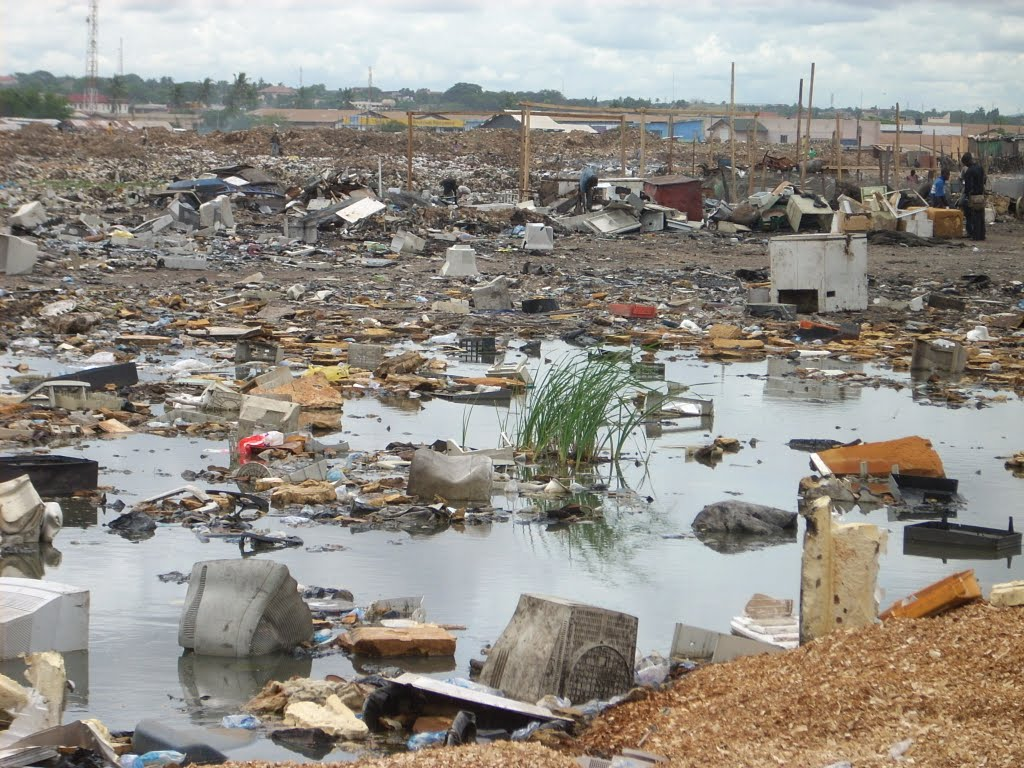
\includegraphics[width=0.5\textwidth]{../inputs/images/ewaste_jack_caravano.jpg}
  \caption{Foto do bairro de Agbogbloshie em Acra. Autorizado por Jack Caravanos, 
           Professor da \textbf{School of Public Health} em \textbf{Hunter College, CUNY}
           Nova Iorque, Estado Unidos da América. \label{fig:ewaste}}
\end{figure}

\citep{ARKU2008} e \citep{DIONISIO2010} foram pioneiros em conduzir  
levantamento dos níveis de poluição, composição elementar e distribuição espacial 
e temporal de poluentes.






